% Manager-side barrier of the distributed GBT training loop. Every Emit* stage in
% learner/distributed_gradient_boosted_trees/distributed_gradient_boosted_trees.cc
% has this shape: fan-out W requests, then pop W replies from one answer queue.
\begin{figure*}[t]
\centering
\begin{minipage}[c]{0.54\textwidth}
\begin{lstlisting}[basicstyle=\ttfamily\scriptsize]
// Manager, one stage (EmitFindSplits, EmitEvaluateSplits, ...)
// fan-out
for (worker_idx = 0; worker_idx < W; ++worker_idx)
  distribute->AsynchronousProtoRequest(request, worker_idx);

// blocks on a queue pop
for (reply_idx = 0; reply_idx < W; ++reply_idx)
  distribute->NextAsynchronousProtoAnswer<proto::WorkerResult>();
\end{lstlisting}
\end{minipage}\hfill
\begin{minipage}[c]{0.44\textwidth}
\centering
\resizebox{\linewidth}{!}{%
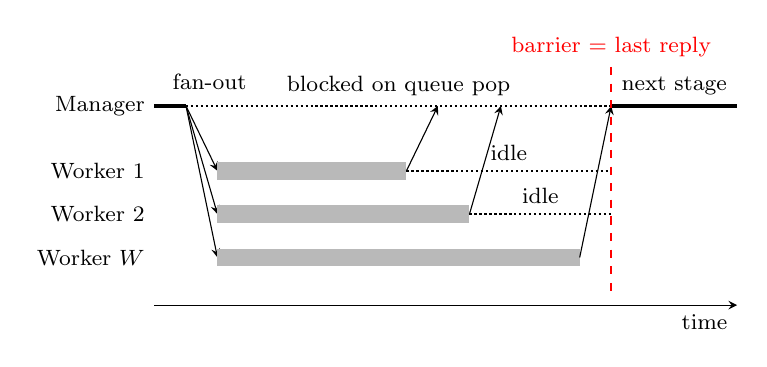
\begin{tikzpicture}[x=1cm, y=0.55cm, >=stealth, font=\footnotesize]
  % swim lanes, slowest worker at the bottom
  \node[anchor=east] at (0,0)    {Manager};
  \node[anchor=east] at (0,-1.5) {Worker 1};
  \node[anchor=east] at (0,-2.5) {Worker 2};
  \node[anchor=east] at (0,-3.5) {Worker $W$};
  \draw[->] (0,-4.6) -- (7.4,-4.6) node[below left] {time};
  % manager: busy, blocked on the queue pop, next stage
  \draw[very thick] (0,0) -- (0.4,0);
  \draw[densely dotted, thick] (0.4,0) -- (5.8,0)
    node[midway, above] {blocked on queue pop};
  \draw[very thick] (5.8,0) -- (7.4,0) node[midway, above] {next stage};
  % fan-out: one request per worker
  \foreach \y in {-1.5,-2.5,-3.5} \draw[->] (0.4,0) -- (0.8,\y);
  \node[above] at (0.7,0.15) {fan-out};
  % worker compute (grey) then idle (dotted) until the barrier
  \fill[gray!55] (0.8,-1.3) rectangle (3.2,-1.7);
  \fill[gray!55] (0.8,-2.3) rectangle (4.0,-2.7);
  \fill[gray!55] (0.8,-3.3) rectangle (5.4,-3.7);
  \draw[densely dotted, thick] (3.2,-1.5) -- (5.8,-1.5) node[midway, above] {idle};
  \draw[densely dotted, thick] (4.0,-2.5) -- (5.8,-2.5) node[midway, above] {idle};
  % replies into the manager's single answer queue
  \draw[->] (3.2,-1.5) -- (3.6,0);
  \draw[->] (4.0,-2.5) -- (4.4,0);
  \draw[->] (5.4,-3.5) -- (5.8,0);
  % the barrier: the last reply is popped
  \draw[dashed, red, thick] (5.8,0.9) node[above] {barrier = last reply} -- (5.8,-4.3);
\end{tikzpicture}}
\end{minipage}
\caption{Manager barrier, one stage of the training loop. Left: the manager
sends one request per worker (fan-out) and then pops $W$ replies from a single
answer queue. Right: grey bars are each worker's compute, dotted segments are
waiting; the next stage starts only after the last reply is popped (dashed
line). The same pattern implements \texttt{StartNewIter}, \texttt{FindSplits},
\texttt{EvaluateSplits}, each \texttt{ShareSplits} round and \texttt{EndIter}.}
\label{fig:manager-barrier}
\end{figure*}
